This chapter covers the modelling of the building blocks of the robot.

\section{Problem statement}
Our robot will be made from a number of elements that all need to be represented in the simulation :\begin{itemize}
\item cameras
\item hands, feet, electronics
\item servos
\end{itemize}

\section{Basic Modelling}
\subsection{Convex elements}
A convex element is an element which has a convex shape, that is, all its interior angles are less or equal to $180\degree$. Our humanoid robot will have some number of them since a lot of elements can be approximated as cubes, which are convex.

The modelling consists in creating a mesh with the right dimensions, setting the mass and setting the inertia (V-Rep does not feature matrix inertias, only principal axes inertias). Friction of the material can also be set and will influence how much an object will slide.

\subsection{Concave elements}
A shape is concave if it is not convex. It is not recommended to use concave shapes in a simulation as they make collision detection more expensive and the simulation is generally more unstable. 

Therefore, the modelling consists in approximating such a shape by several convex shapes, linked together.

\section{Applied to the building of a humanoid robot}
\subsection{Feet}
The shape of the feet is not fixed yet but it is safe to approximate them by a convex shape with high friction. 

\subsection{Frames}
The frames in use, FR07-H101 are convex and are thus decomposed into into convex shapes 
that are linked together. 

\subsection{Eletronics}
Electronics 

\subsection{Cameras}
Cameras are modelled as cubes. Their function is performed by vision sensors handled by V-Rep.
\begin{figure}[htp]
\center
    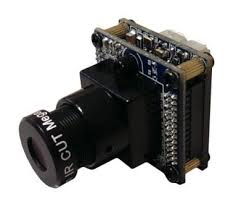
\includegraphics[width = 0.3\textwidth]{figures/li_cam}
    \caption{LI-USB30-M021C camera, to be used in the robot.}
    \label{fig:camera}
\end{figure}

\subsection{Servos}
\begin{figure}[htp]
\center
\begin{subfigure}[b]{0.3\textwidth}
    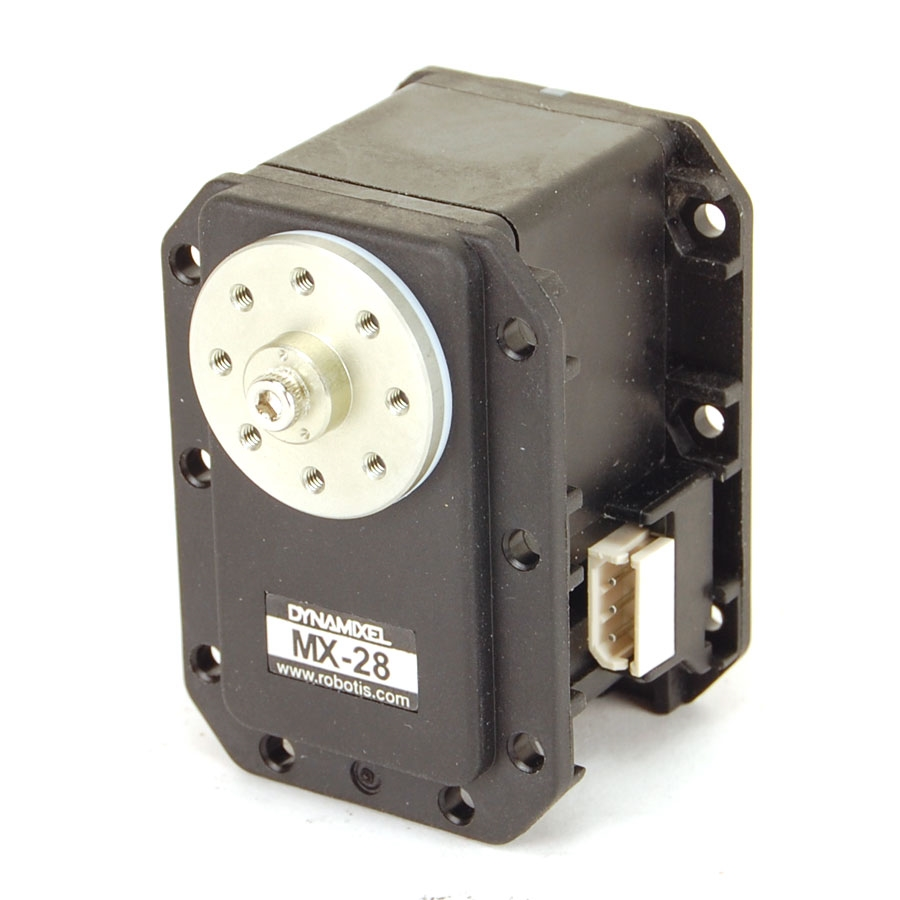
\includegraphics[width = \textwidth]{figures/mx28}
    \caption{MX-28R servo.}
    \label{fig:mx28}
\end{subfigure}
\hfill
\begin{subfigure}[b]{0.3\textwidth}
    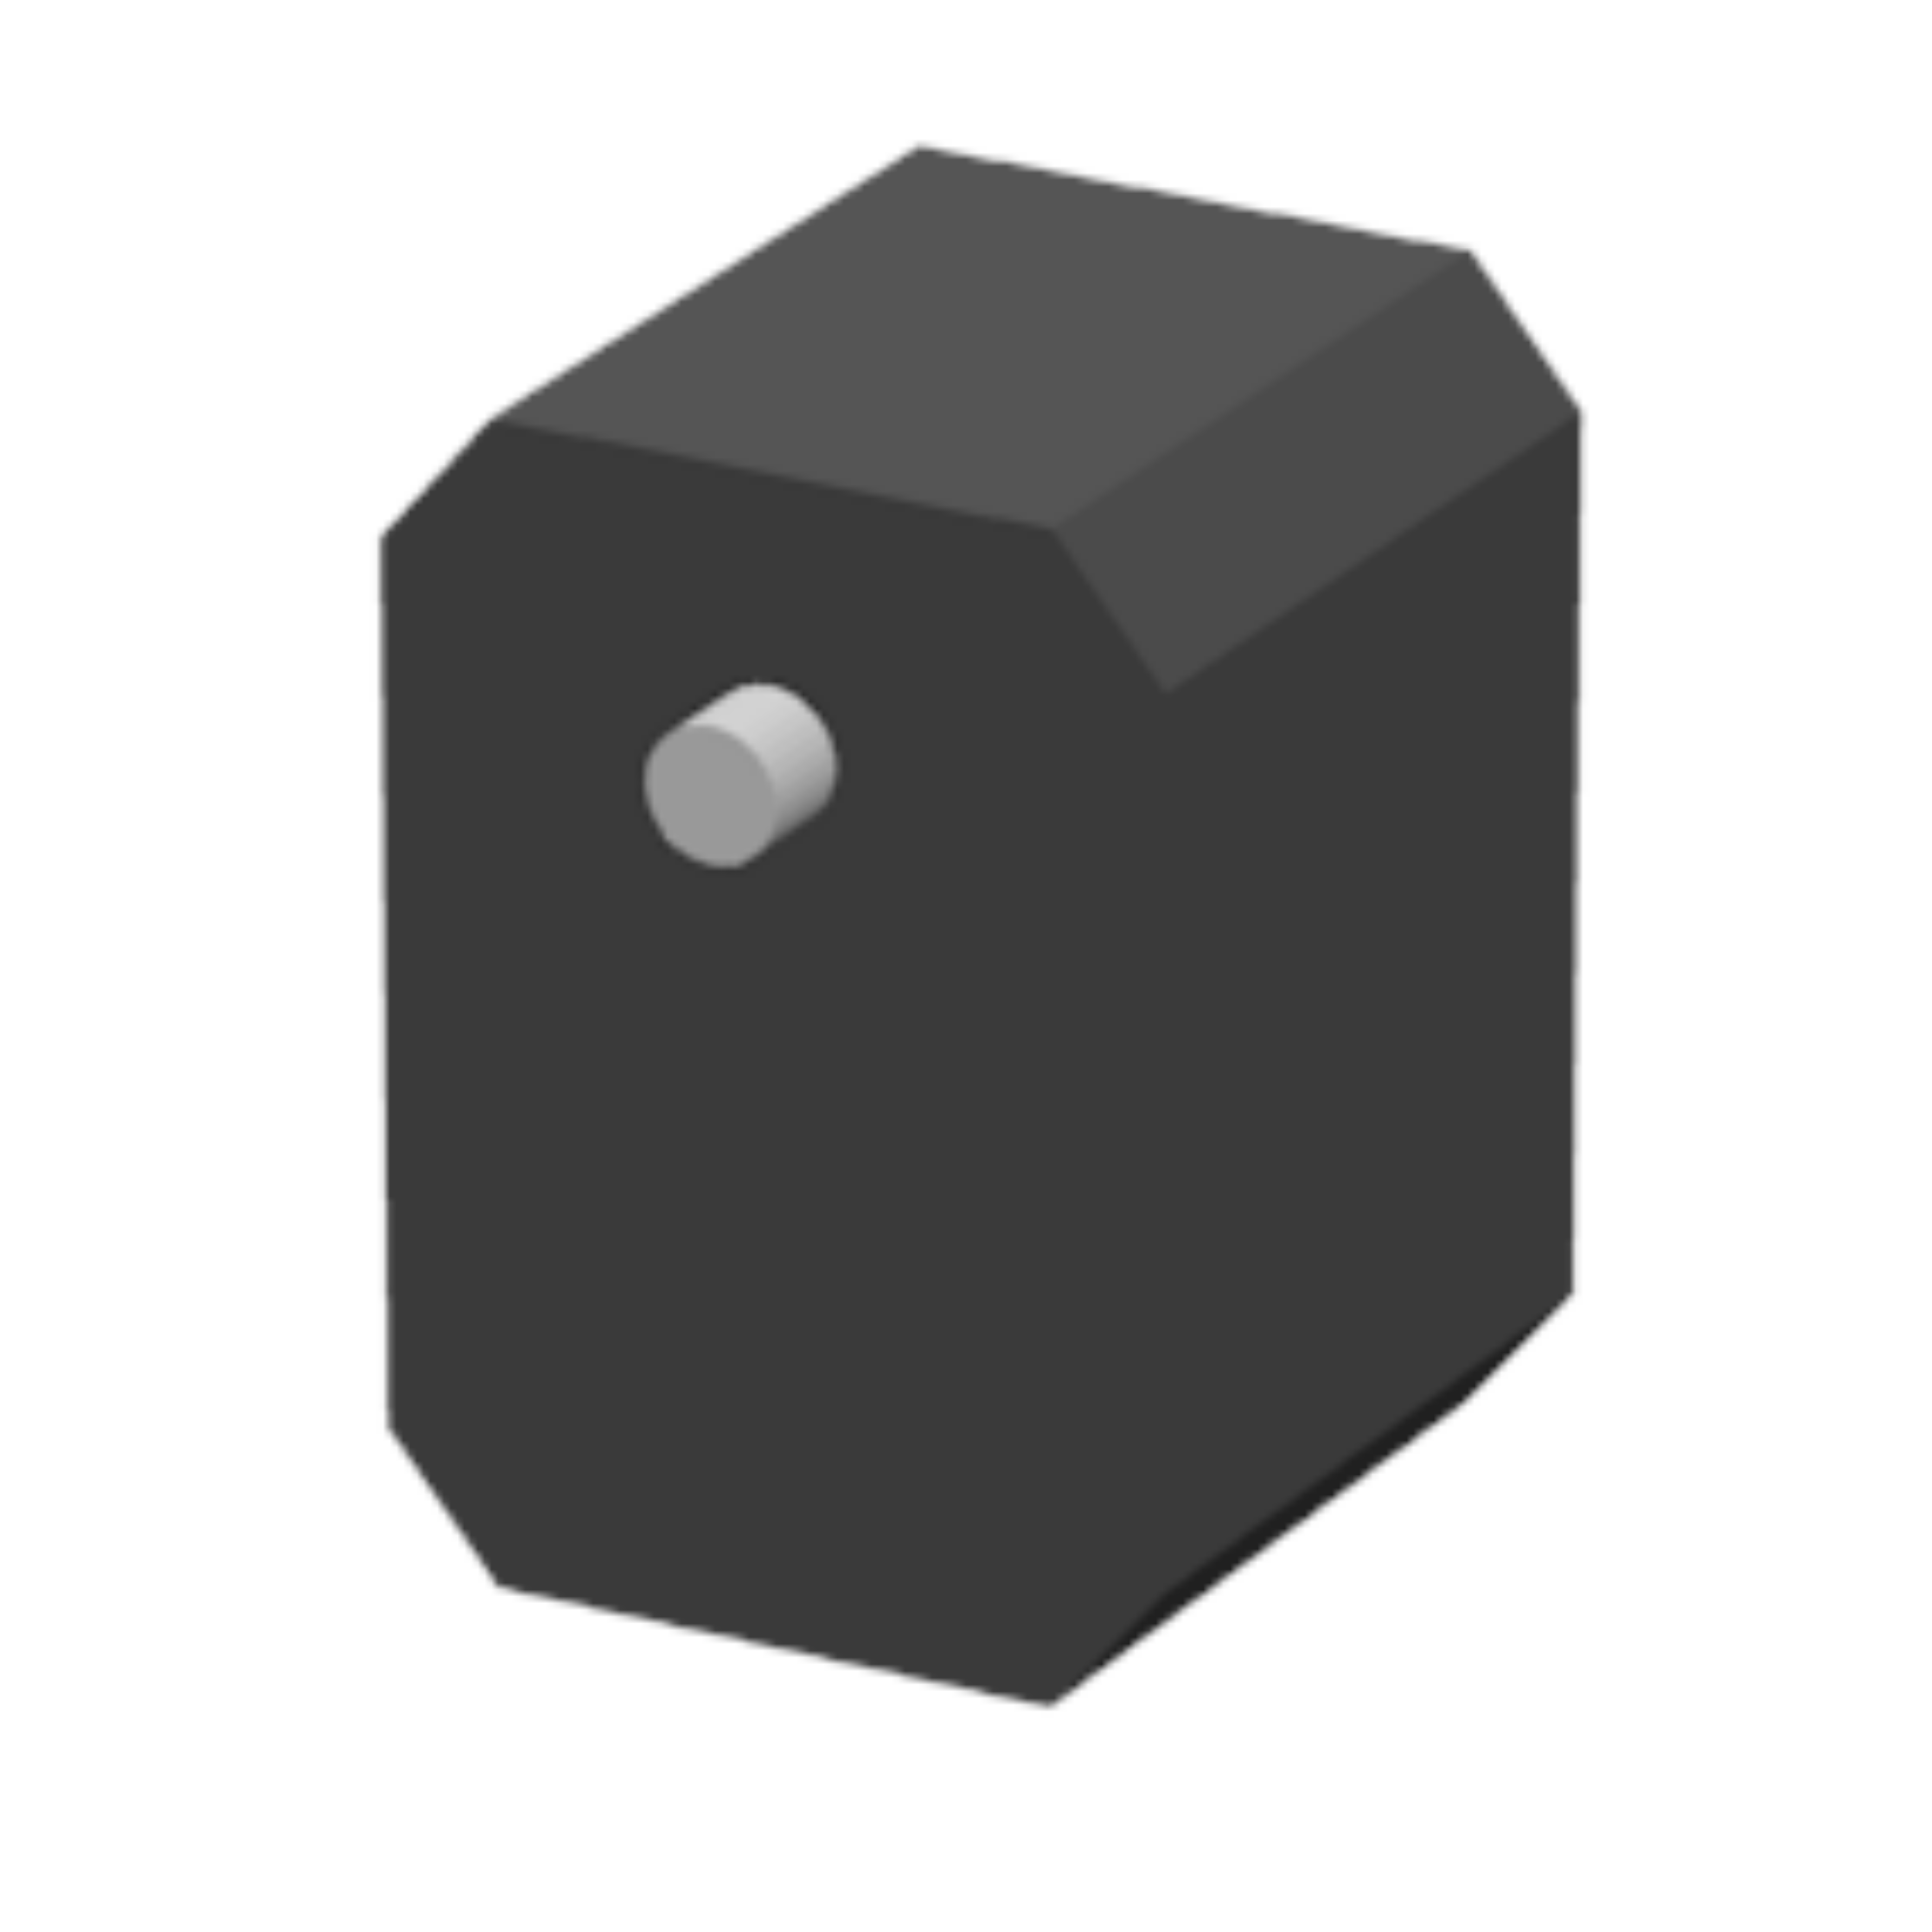
\includegraphics[width = \textwidth]{figures/mx28_model}
    \caption{Model of the MX-28R.}
    \label{fig:mx28_model}
\end{subfigure}
\caption{Side by side of a MX-28R servo and its 3D model. The shape has been simplified but retains outer appearance of the servo. The axis is used as a position marker and will be removed once the joints are in place.}
\label{fig:servo}
\end{figure}

The robot will mainly be made from MX-28R servos, manufactured by Dynamixel. Their size and power make them an good choice for a humanoid robot. The goal of this section is thus to reproduce as accurately as possible the behaviour of this servo in our simulation.

The MX-28R outer shape is convex so we can create a convex mesh to model its appearance. Its mass and inertias can be set to $77g$ and 
\begin{align*}
Ixx Iyy Izz = (
\end{align*}

\begin{table}[htp]
\center
\begin{tabularx}{\textwidth}{@{} l l l @{}}
\toprule
& \textbf{Data} & \textbf{Unit}\\ 
\midrule
Weight & $77$ & $g$\\
Dimension & $35.6 \times 50.6 \times 35.5$ & $mm^3$\\
Inertia around main axes & $(\begin{array}{c c c}
33,765 & 12,900 & 28,821
\end{array})$ & $g \times mm^4$ \\
Stall torque & $2.5$ & $Nm$\\
Nominal torque & $0.7$ & $Nm$\\
\bottomrule
\end{tabularx}
\caption{Characteristics of a MX-28R type servo. Data taken from \cite{mx_28_manual}}
\label{table:specs}
\end{table}

The torque of the servos is computed from the maximal torque of the DC motor and the reduction ratio of the gears. 
\begin{align*}
Torque &= TorqueMotor \times ReductionRatio\\
&= 3.67e^{-3} \times 193\\
&= 0.7083Nm
\end{align*} 

\begin{lstlisting}[language={[5.0]Lua}, numbers = left, tabsize = 4, frame=leftline, keywordstyle=\color{blue}, float, caption=Control code of the servo, captionpos = b ]
-- init: true when this callback is called for the first time (if the joint is dynamically reset during the simulation, this might be true more often)
-- revolute: true if the joint is revolute
-- cyclic: true if the joint is revolute and cyclic (i.e. no lower/upper limits)
-- currentPos: the current position of the joint
-- targetPos: the desired position of the joint
-- errorValue: targetPos-currentPos (with revolute cyclic joints we take the shortest cyclic distance)
-- effort: the last force or torque that acted on this joint along/around its axis. With Bullet, torques from joint limits are not taken into account
-- dynStepSize: the step size used for the dynamics calculations (by default 5ms)
-- lowLimit: the joint lower limit
-- highLimit: the joint upper limit
-- targetVel: the joint target velocity (as set in the user interface)
-- maxForceTorque: the joint maximum force/torque (as set in the user interface)
-- velUpperLimit: the joint velocity upper limit (as set in the user interface)

if not PID_P then
    PID_P=0.1
    PID_I=0
    PID_D=0
end

if init then
    pidCumulativeErrorForIntegralParam=0
end
ctrl = errorValue*PID_P

if PID_I ~=0 then
    pidCumulativeError = pidCumulativeError+errorValue*dynStepSize
else
    pidCumulativeErrorForIntegralParam=0
end

ctrl=ctrl+pidCumulativeError*PID_I
if not init then
    ctrl=ctrl+(errorValue-pidLastError)*PID_D/dynStepSize
end
pidLastError=errorValue

velocityToApply=ctrl/dynStepSize
if (velocityToApply>velUpperLimit) then
    velocityToApply=velUpperLimit
end
if (velocityToApply<-velUpperLimit) then
    velocityToApply=-velUpperLimit
end
forceOrTorqueToApply=maxForceTorque

return forceOrTorqueToApply,velocityToApply
\end{lstlisting}

\subsection{Springs}

